Como parte fundamental de la creación de un SRI se tiene el proceso de
evaluación, donde se determinará la eficacia del mismo.

Para la evaluación del modelo propuesto se cuenta, como procedimiento estándar,
con varias colecciones de pruebas, las cuales contienen lo siguiente:

\begin{enumerate}
    \item Una colección de documentos.
    \item Un conjunto de pruebas a realizar sobre la colección, llamadas
    consultas (\emph{queries}).
    \item Un conjunto de juicios de relevancia, una evaluación mayormente
    binaria sobre la relevancia de las consultas sobre los documentos (en
    algunas de las colecciones utilizadas el espectro de evaluación no es tan
    binario) 
\end{enumerate}

Sobre la estructura de las colecciones utilizadas y descritas con anterioridad,
trabaja el modelo, se realizan comparaciones y cálaculo de métricas que
caracterizan la efectividad del mismo.

\subsection{Proceso de Evaluación}

Para el proceso de evaluación se analiza la siguiente estructura (a modo de
ejemplo), resultante del proceso de recuperación del modelo.

\begin{figure}[h!]%
    \centering
	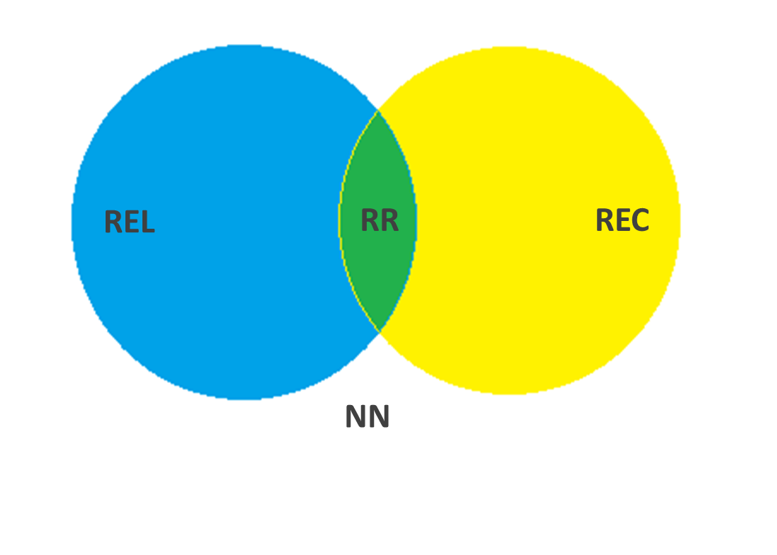
\includegraphics[width=0.4\textwidth]{./sri_03.png}
	\caption{Clasificación de los documentos después de una consulta.}
	\label{fig:docSet}
\end{figure}

Donde:
\begin{itemize}
    \item {\bf REL:} Conjunto de documentos relevantes.
    \item {\bf REC:} Conjunto de documentos recuperados.
    \item {\bf RR:} Conjunto de documentos relevantes recuperados.
    \item {\bf NN:} Conjunto de documentos no relevantes no recuperados.
\end{itemize}

Para un mejor analisis de la relevancia, aunque partimos de la estructura
anterior, se hace preciso el uso de nuevos conjuntos, a la par de los ya
definidos.

\begin{itemize}
    \item RI: Conjunto de documentos recuperados irrelevantes (REC$-$RR)
    \item NR: Conjunto de documentos no recuperados relevantes (REL$-$RR)
\end{itemize}

Sobre esta partición de conjuntos se aplican varias medidas de evaluación, con
las cuales se verifican la efectividad del modelo.

\subsubsection{Métricas estándares}



\begin{itemize}
\item Precisión:
    $$P = \dfrac{|RR|}{|RR \cup RI|}$$
    Denota la calidad de la respuesta y la clasificación. A medida que aumenten
    las cantidad de documentos de la colección y, por tanto, los documentos
    recuperados, esta medida sea menor.\\
\item Recobrado (Recall):
    $$R = \dfrac{|RR|}{|RR \cup NR|}$$
    A diferencia de la Precisión, esta medida aumenta mientras más documentos
    se incorporan a la respuesta.\\
\item Medida F:
    $$F = \dfrac{(1+\beta^2)PR}{\beta^2P+R} = \dfrac{1+\beta^2}{\frac{1}{P}+
    \frac{\beta^2}{R}}$$
    Medida para enfatizar la Precisión contra el Recobrado o viceversa.
    \begin{itemize}
    \item $\beta =1$ Igual peso para la Precisión y el Recobrado ($F=F_1$).
    \item $\beta >1$ Mayor peso para la Precisión.
    \item $\beta =1$ Mayor peso para el Recobrado.\\
    \end{itemize}
\item Medida $F_1$:
    $$F_1 = \dfrac{2PR}{P+R} = \dfrac{2}{\frac{1}{P} + \frac{1}{R}}$$
    Medida que armoniza entre Precisión y Recobrado.
\end{itemize}

Estas medidas, aunque efectivas, no tienen en cuanta el \emph{ranking} de los
documentos, por lo que para una mayor efectividad del modelo se emplean otras
dos medidas para un mejor rendimiento.

\subsubsection{Métricas Dependientes del \emph{Ranking}}

\begin{itemize}
    \item R-Precisión:
    La R-Precisión consiste en aplicar la fórmula de Precisión a partir de la
    posición $R$ del ranking de documentos relevantes.\\
    \item Fallout:
        $$Fallout = \dfrac{|RI|}{|RI\cup NN|}$$
\end{itemize}

Se incluyen en el modelo, además, opciones de comparación entre varias
colecciones, con el fin de realizar análisis entre las mismas.